% -*- latex -*-
%%%%%%%%%%%%%%%%%%%%%%%%%%%%%%%%%%%%%%%%%%%%%%%%%%%%%%%%%%%%%%%%
%%%%%%%%%%%%%%%%%%%%%%%%%%%%%%%%%%%%%%%%%%%%%%%%%%%%%%%%%%%%%%%%
%%%%
%%%% This text file is part of the source of 
%%%% `Parallel Programming in MPI and OpenMP'
%%%% by Victor Eijkhout, copyright 2012-6
%%%%
%%%% affinity.tex : about process and thread affinity
%%%%
%%%%%%%%%%%%%%%%%%%%%%%%%%%%%%%%%%%%%%%%%%%%%%%%%%%%%%%%%%%%%%%%
%%%%%%%%%%%%%%%%%%%%%%%%%%%%%%%%%%%%%%%%%%%%%%%%%%%%%%%%%%%%%%%%

\index{affinity!process and thread|(}

In the preceeding chapters we mostly considered all MPI nodes or
OpenMP thread as being in one flat pool.
However, for high performance you need to worry about \indextermdef{affinity}:
the question of which process or thread is placed where, and how
efficiently they can interact.

\begin{figure}[ht]
  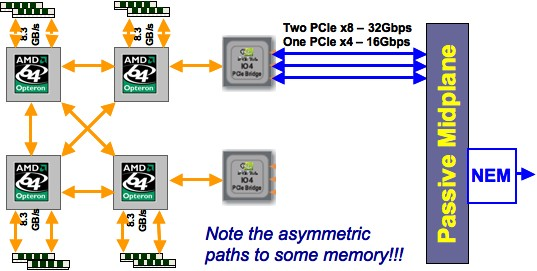
\includegraphics[scale=.7]{ranger-numa}
  \caption{The NUMA structure of a Ranger node}
  \label{fig:ranger-numa}
\end{figure}

Here are some situations where you affinity becomes a concern.
\begin{itemize}
\item In pure MPI mode processes that are on the same node can
  typically communicate faster than processes on different
  nodes. Since processes are typically placed sequentially, this means
  that a scheme where process~$p$ interacts mostly with $p+1$ will be
  efficient, while communication with large jumps will be less so.
\item If the cluster network has a structure
  (\indextermsub{processor}{grid} as opposed to \indexterm{fat-tree}),
  placement of processes has an effect on program efficiency.  MPI
  tries to address this with \indexterm{graph topology};
  section~\ref{sec:mpi-dist-graph}.
\item Even on a single node there can be
  asymmetries. Figure~\ref{fig:ranger-numa} illustrates the structure
  of the four sockets of the \indexterm{Ranger} supercomputer (no
  longer in production). Two cores have no direct connection.

  This asymmetry affects both MPI processes and threads on that node.
\item Another problem with multi-socket designs is that each socket
  has memory attached to it. While every socket can address all the
  memory on the node, its local memory is faster to access. This
  asymmetry becomes quite visible in the \indexterm{first-touch}
  phenomemon; section~\ref{sec:first-touch}.
\item If a node has fewer MPI processes than there are cores, you want
  to be in control of their placement. Also, the operating system can
  migrate processes, which is detrimental to performance since it
  negates data locality. For this reason, utilities such as
  \indextermtt{numactl}
\begin{tacc}
(and at TACC \indextermtt{tacc_affinity})    
\end{tacc}
  can be used to \indexterm{pin a thread} or process to a specific core.
\item Processors with \indexterm{hyperthreading} or
  \indextermsub{hardware}{threads} introduce another level or worry
  about where threads go.
\end{itemize}

\Level 0 {What does the hardware look like?}

If you want to optimize affinity, you should first know what the
hardware looks like. The \indextermttdef{hwloc} utility is valuable
here~\cite{goglin:hwloc} (\url{https://www.open-mpi.org/projects/hwloc/}).

\begin{figure}[ht]
  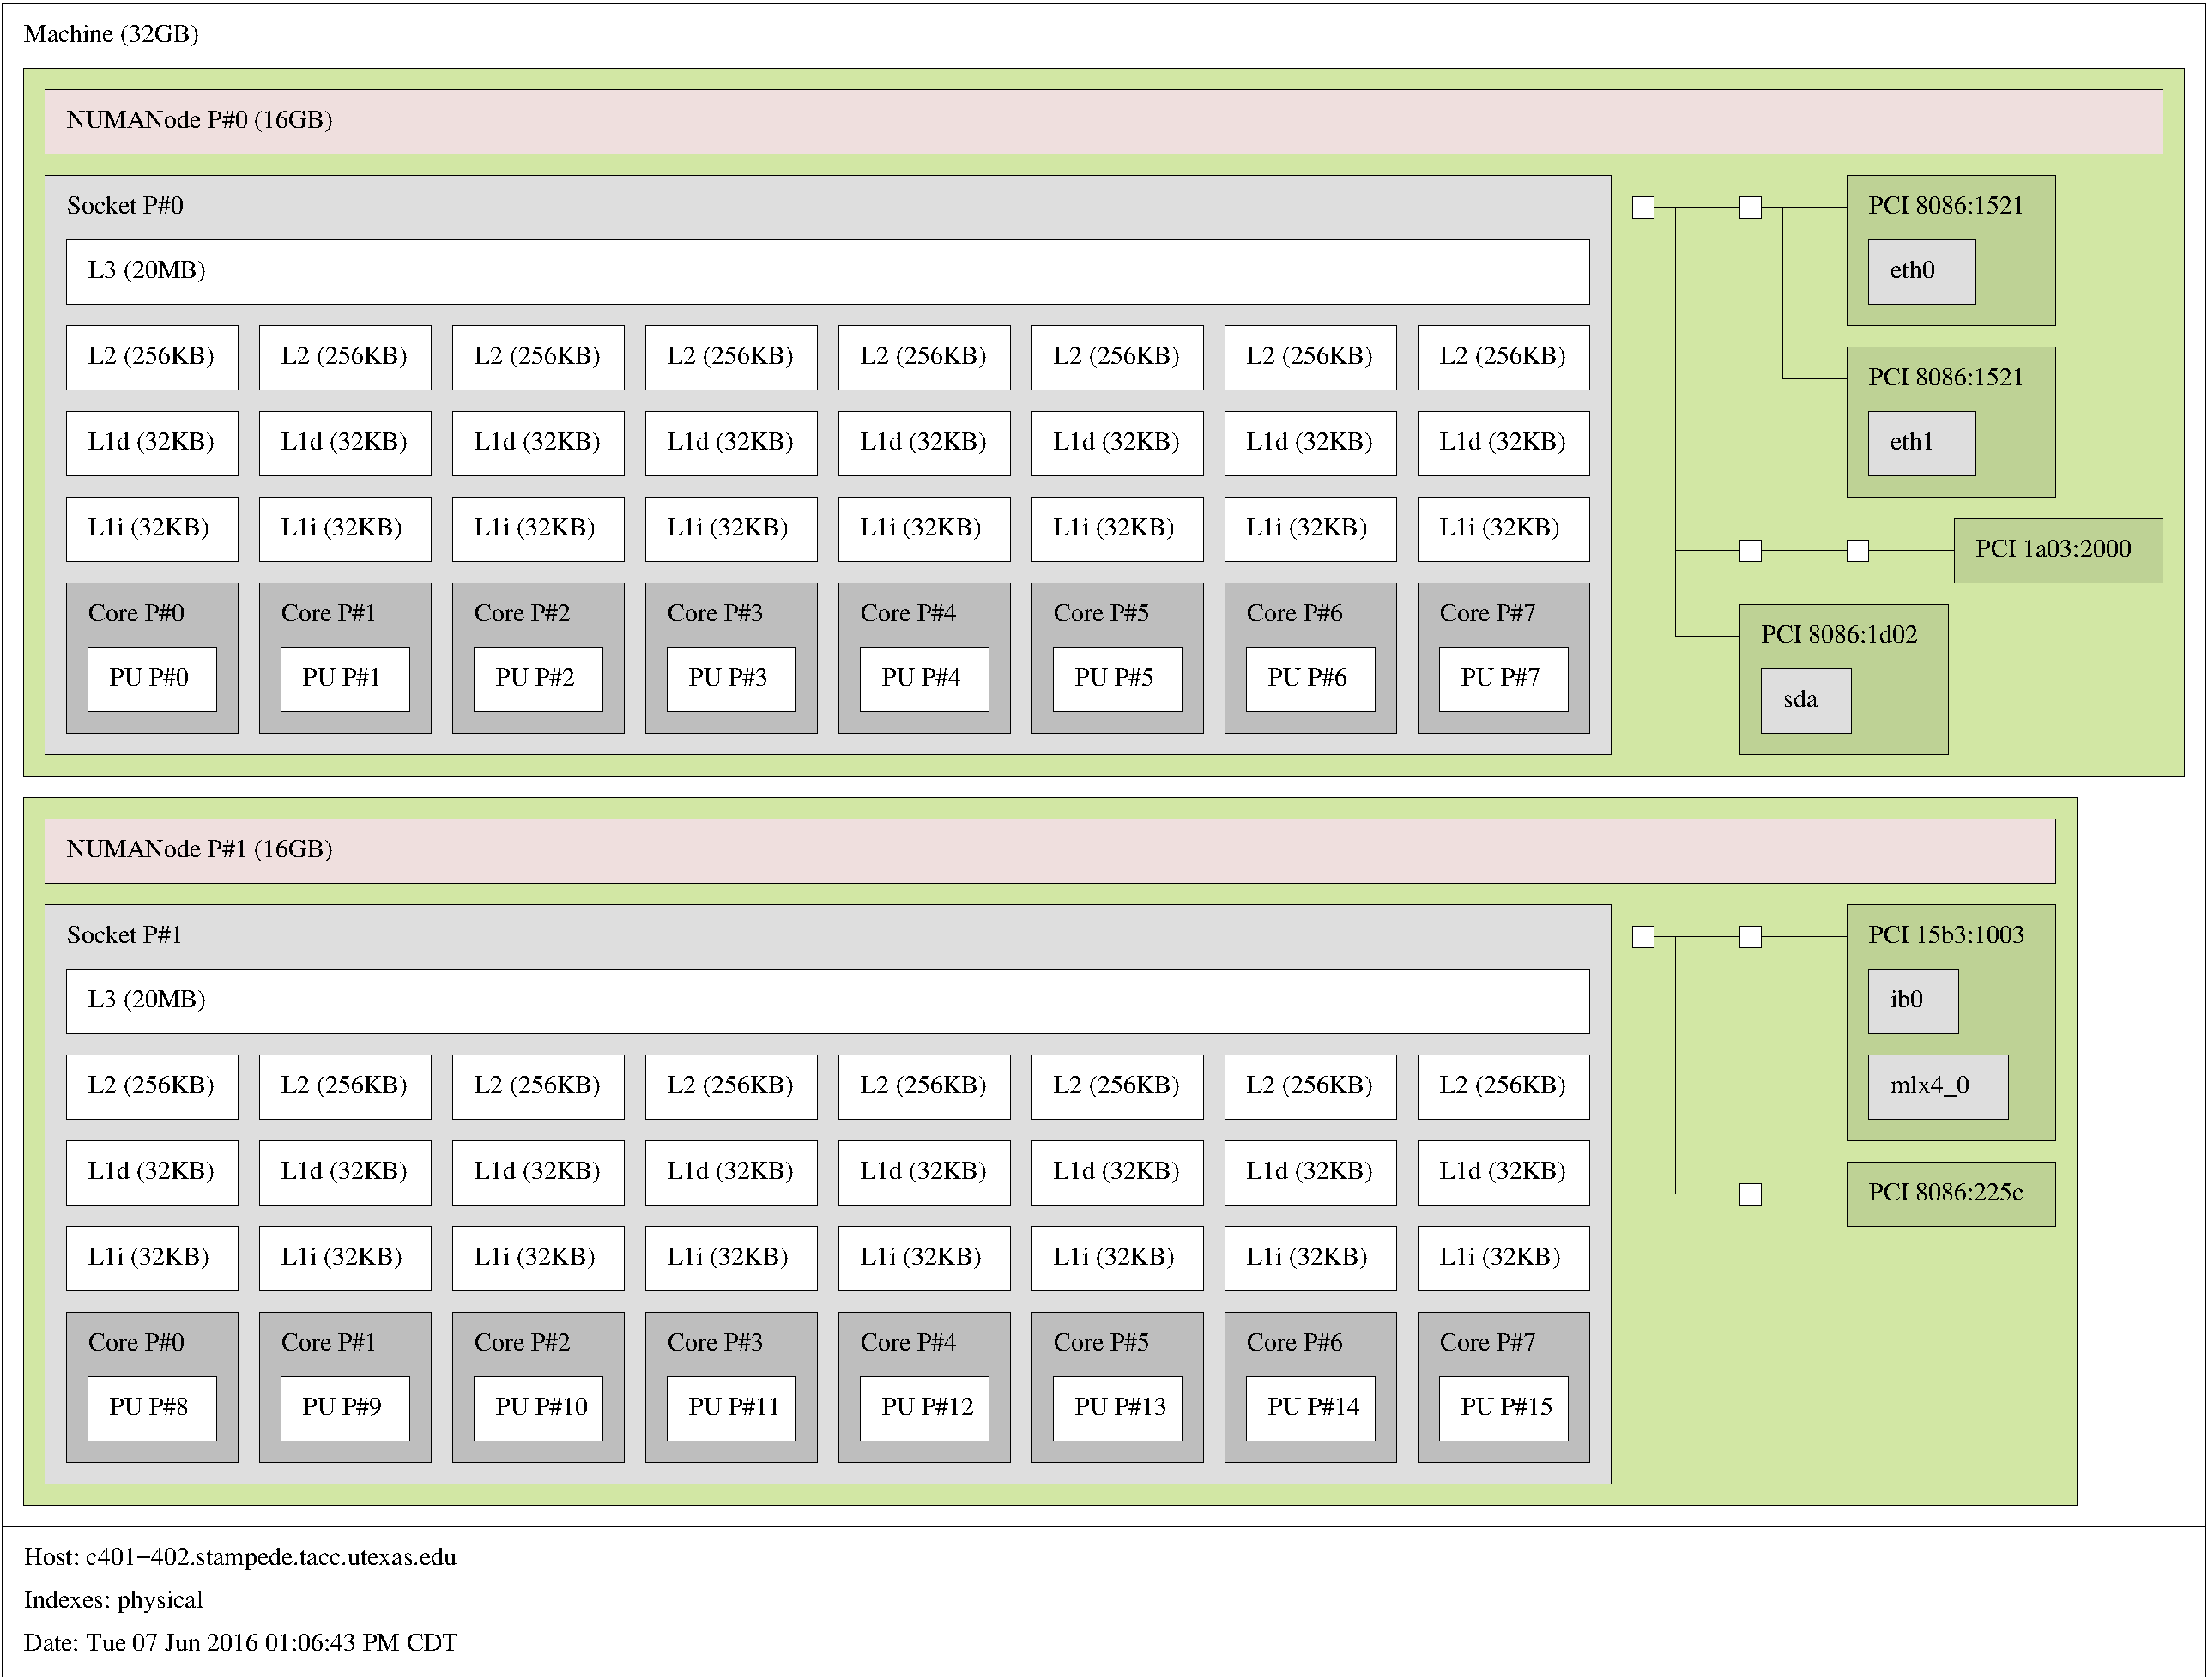
\includegraphics[scale=.3]{stampede-compute}
  \caption{Structure of a Stampede compute node}
  \label{fig:stampede-compute-hwloc}
\end{figure}

\begin{figure}[p]
  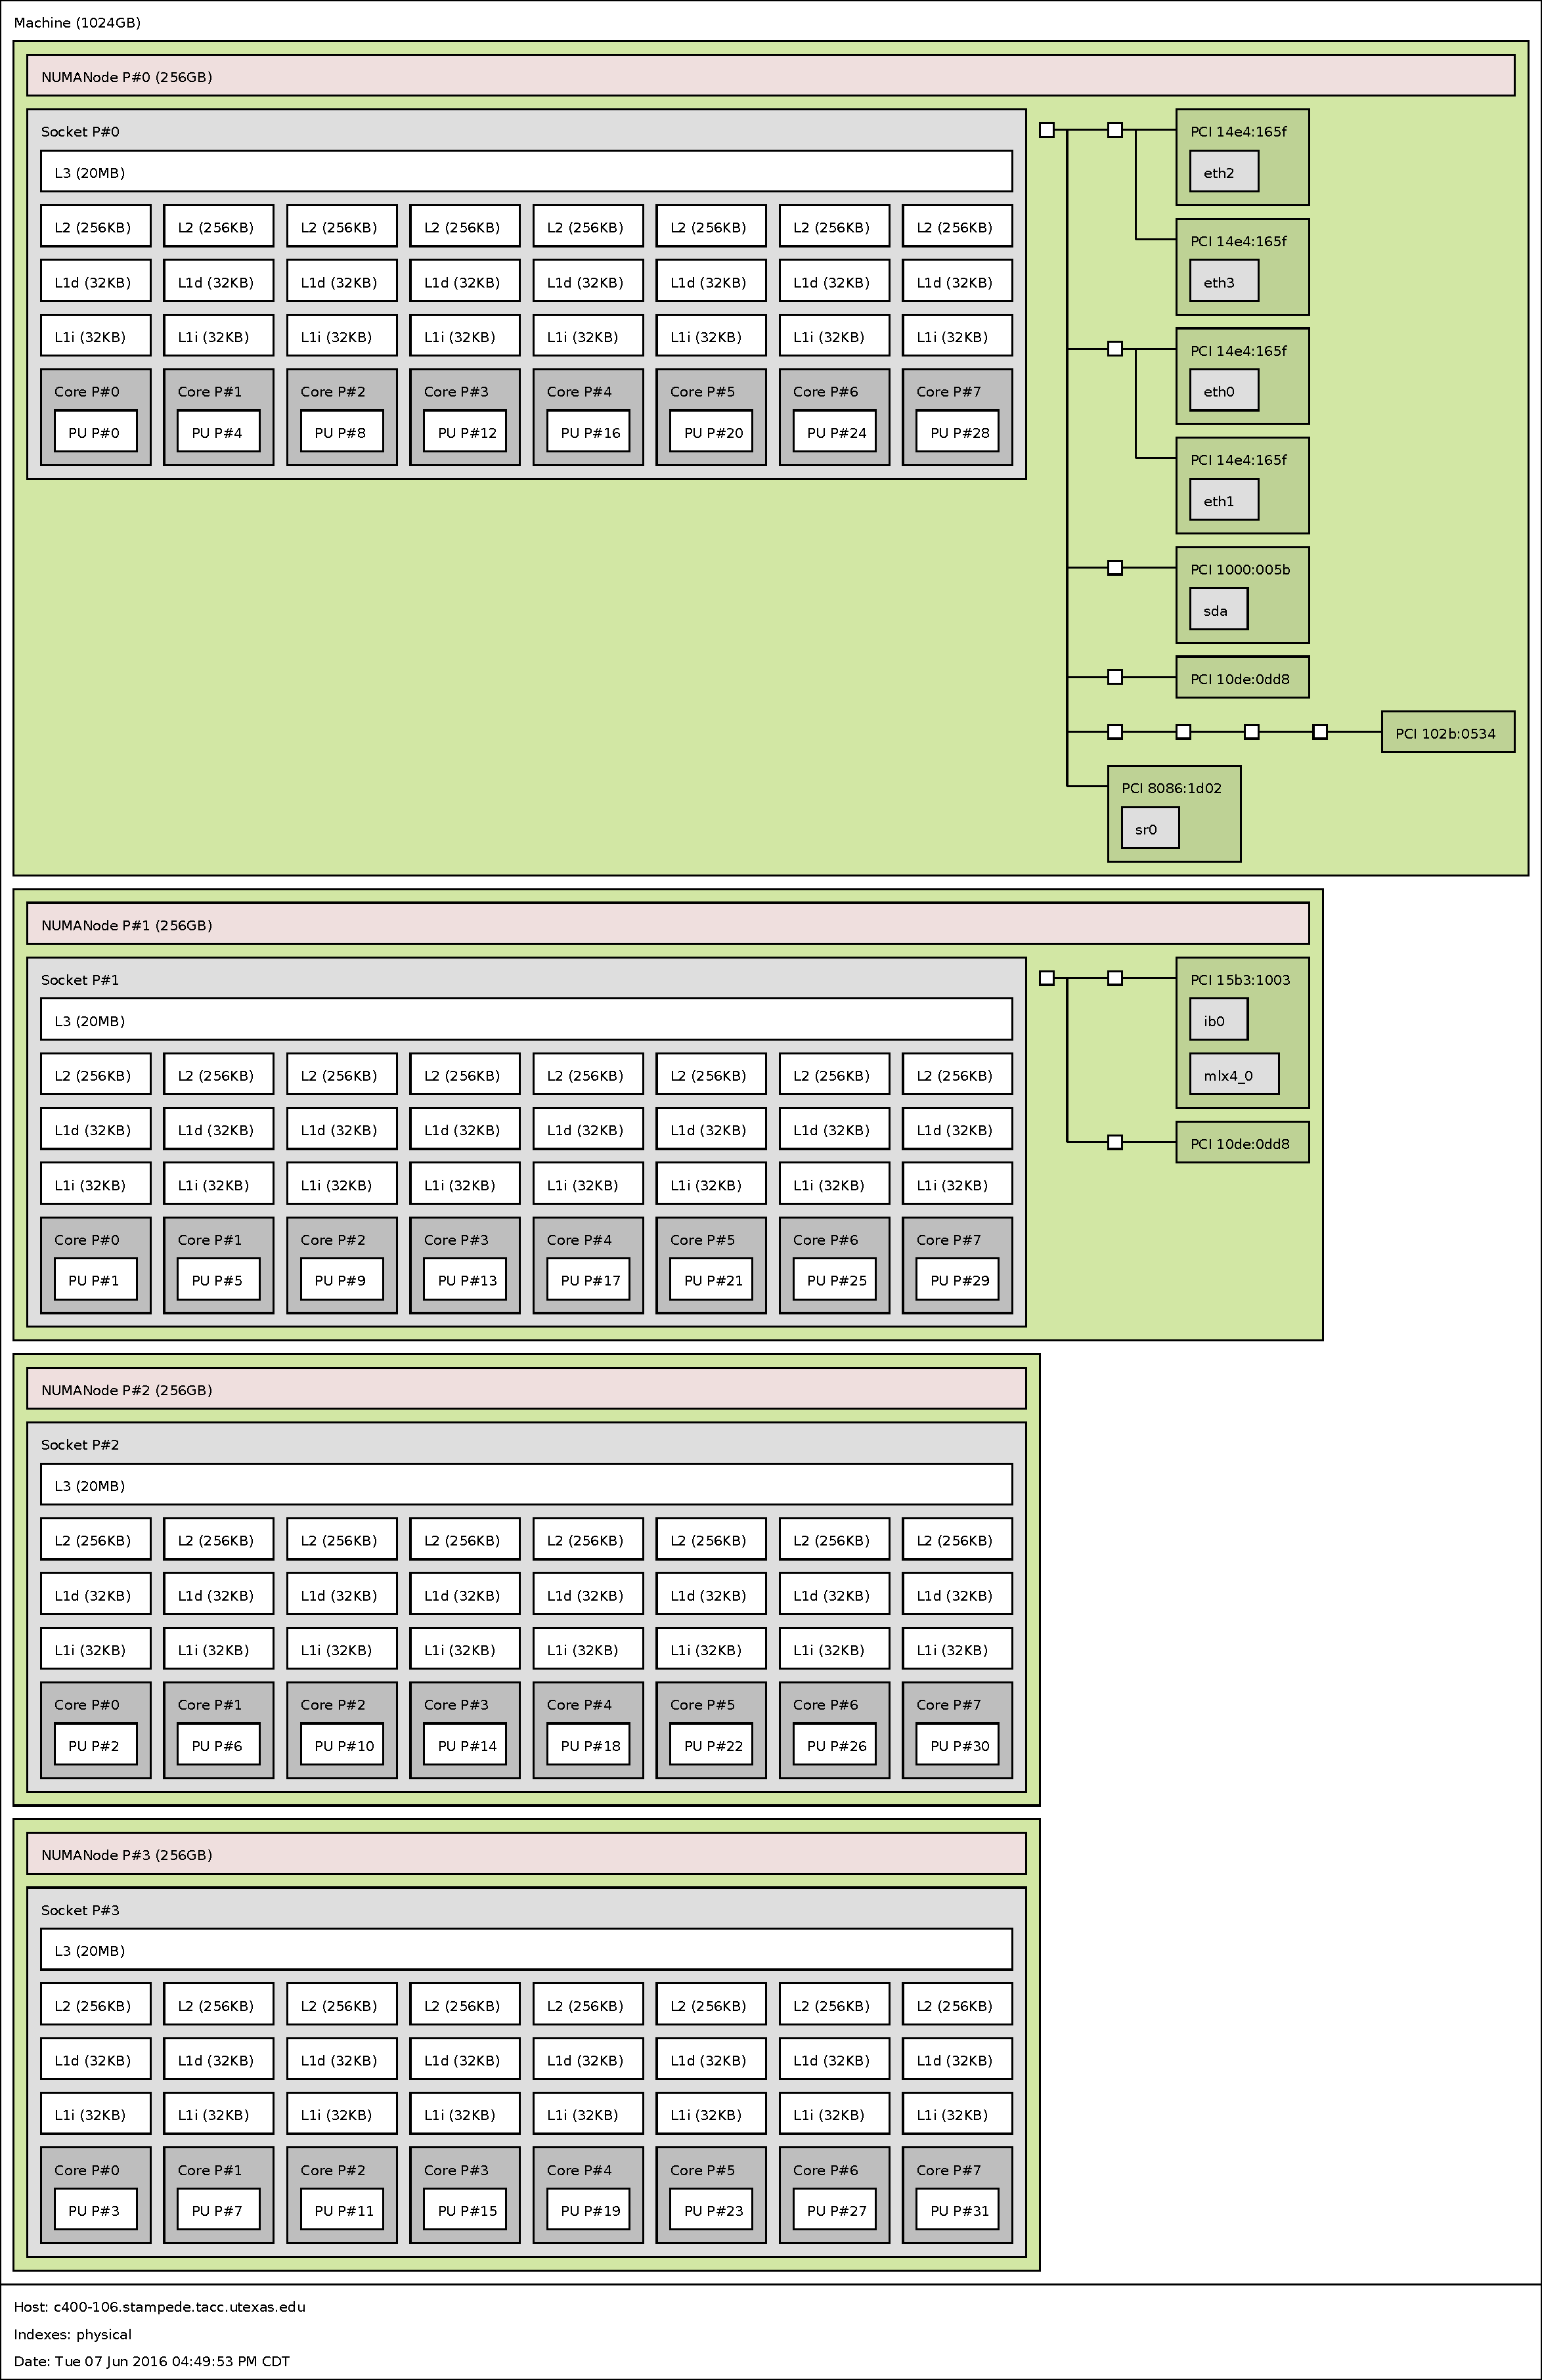
\includegraphics[scale=.3]{stampede-largemem}
  \caption{Structure of a Stampede largemem four-socket compute node}
  \label{fig:stampede-largemem-hwloc}
\end{figure}

\begin{figure}[ht]
  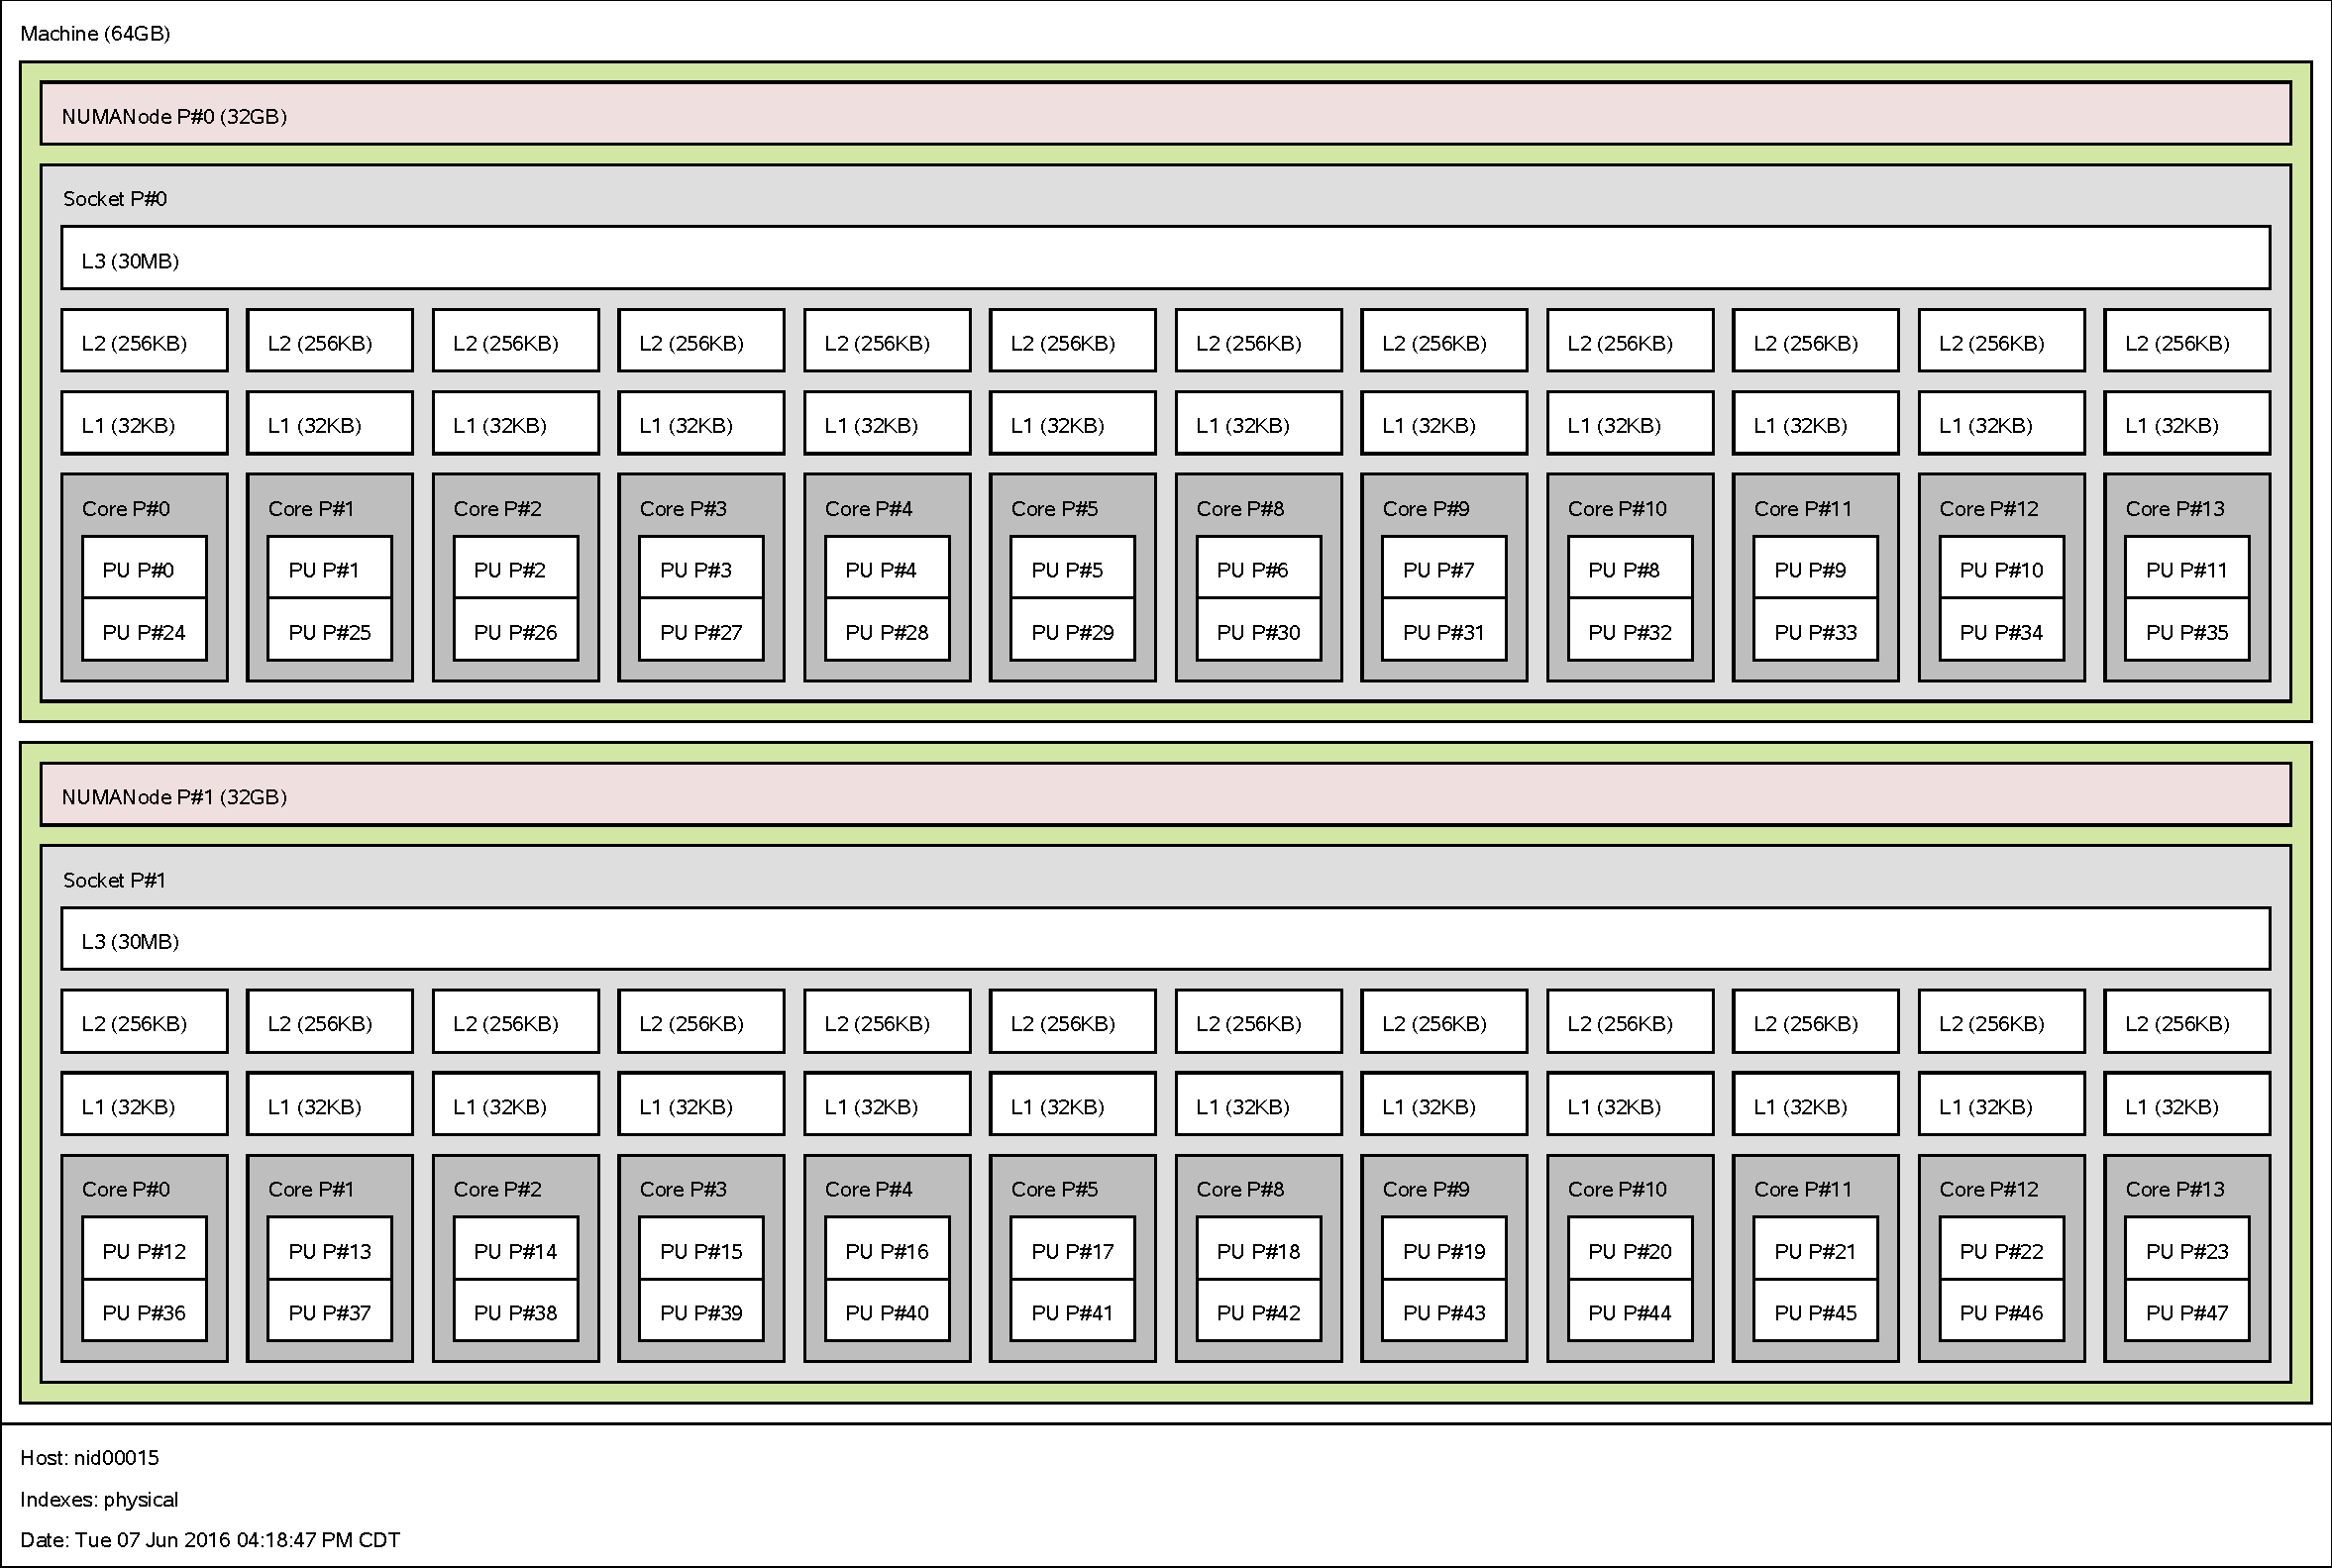
\includegraphics[scale=.3]{ls5}
  \caption{Structure of a Lonestar5 compute node}
  \label{fig:ls5-compute-hwloc}
\end{figure}

Figure~\ref{fig:stampede-compute-hwloc} depicts a
\indextermbus{Stampede}{compute node}, which is a two-socket
\indextermbus{Intel}{SandyBridge} design;
figure~\ref{fig:stampede-largemem-hwloc} shows a 
\indextermbus{Stampede}{largemem node}, which is a four-socket design.
%
Finally, figure~\ref{fig:ls5-compute-hwloc} shows a
\indexterm{Lonestar5} compute node, a~two-socket design with 12-core
\indextermbus{Intel}{Haswell} processors with two hardware threads
each.

\Level 0 {Affinity control}

See chapter~\ref{ch:omp-affinity} for OpenMP affinity control.

\index{affinity!process and thread|)}
